% ch9.tex
% This work is licensed under the Creative Commons Attribution-Noncommercial-Share Alike 3.0 New Zealand License.
% To view a copy of this license, visit http://creativecommons.org/licenses/by-nc-sa/3.0/nz
% or send a letter to Creative Commons, 171 Second Street, Suite 300, San Francisco, California, 94105, USA.


\chapter{Um pouco sobre gráficos}\label{ch:abitgraphic}

O problema de usar a tartaruga para desenhar, é$\ldots$ que$\ldots$$\ldots$ as tartarugas$\ldots$$\ldots$$\ldots$ são$\ldots$$\ldots$$\ldots$$\ldots$muito$\ldots$$\ldots$$\ldots$$\ldots$ lentas.
\par
Mesmo quando uma tartaruga está no seu máximo de velocidade, ela ainda não está indo rápido. Para tartarugas, isso não é um problema --- eles tem tempo a perder ---- mas quando estamos falando de gráficos de computador, isso é um problema. Se você tem um Nintendo DS, um Gameboy Advance ou jogos no seu computador, pense por um momento sobre os gráficos (que você vê na tela). Existem diversas formas de exibição de gráficos que são usadas em jogos: existem os jogos 2d (ou de 2 dimensões), onde as imagens são planas e os personagens geralmente se movem para cima, para baixo, esquerda e direita --- muitoc omum em videogames de mão --- e finalmente, os jogos 3d, onde as figuras desenhadas na tela tentando imitar a realidade.

Todos estes tipos de gráficos tem uma coisa em comum --- eles precisam ser desenhados muito rapidamente. Você já tentou fazer a sua própria animação? Onde você pega um bloco de folhas de papel e no canto, na parte debaixo da primeira página, e na próxima folha, você desenha a figura um pouco mais para frente e por assim em diante. Quando você terminar, você folheia as páginas e se você folhear rápido o suficiente, vai parecer que a figura está realmente se movendo. É assim que basicamente todas as animações são feitas --- se forem os desenhos que você assiste na tv ou os jogos que você joga no videogame ou computador. Você desenha algo e depois desenha a mesma coisa novamente, com pequenas mudanças, para dar a ilusão de movimento. Que é o motivo pelo qual a tartaruga não é tão boa fazendo gráficos. Para fazer uma imagem parecer que está se movendo, você precisa desenhar cada `frame' (quadro) da animação muito rapidamente.
\par
Gráficos tridimensionais são feitos de uma maneira bem diferente dos gráficos bidimensionais, mas ainda assim, a ideia básica é a mesma. No momento em que a sua tartaruga terminou de desenhar uma pequena porção de uma figura, já seria hora de virar a página e começar a desenhar a próxima$\ldots$

\begin{center}
\includegraphics*[width=100mm]{eps/turtle1.eps}
\end{center}

\section{Desenhar rapidamente}

Cada linguagem de programação tem um método diferente de desenhar na tela. Alguns métodos são mais rápidos, enquanto outros são mais lentos, o que significa que os programadores que criam jogos tem que ser cuidadosos na hora de escolher a linguagem que vão usar para trabalhar.
\par
Assim como o Python também possui diversas formas diferentes de fazer gráficos (incluindo a tartaruga, que nós já usamos), mas os melhores métodos (do ponto de vista dos gráficos) normalmente são módulos e bibliotecas que são incluidas no Python por padrão. Você provavelmente terá que programar por alguns anos para poder instalar e usar algumas dessas bibliotecas complexas.

Felizmente, existe um módulo que vem com o Python, que podemos usar para fazer gráficos simples (um pouco mais rápido que a tartaruga). Talvez rápida o suficiente para a chamarmos de Tartaruga Rápida para Desenhar.

\begin{center}
\includegraphics*[width=100mm]{eps/turtle2.eps}
\end{center}

O módulo se chama \code{tkinter}\index{modules!tkinter} (um nome estrenho, que vem de `Tk interface') e pode ser usada para criar aplicações completas (você pode até mesmo criar um Editor de Textos se quiser), assim como apenas desenhar. Nós podemos criar uma aplicação simples com um botão, usando o seguinte código:

\begin{listing}
\begin{verbatim}
1. >>> from tkinter import *
2. >>> tk = Tk()
3. >>> btn = Button(tk, text="clique aqui")
4. >>> btn.pack()
\end{verbatim}
\end{listing}

In line 1,  we import the contents of the \code{Tk} module, so we can use them---the most useful of these is \code{Tk}, which creates a basic window to which we can then add things. After you type in line 2, that window will suddenly appear on the screen.  In line 3, we create a new Button and assign it to the variable \code{btn}. The button is created by passing the \code{tk} object as a parameter, along with a named parameter with the words `click me'.

\par
\fbox{\colorbox{PaleBlue}{\parbox{.75\linewidth} {
\section*{Named Parameters}

This is the first time we've used `named parameters'\index{named parameters}. These work just like normal parameters, except they can appear in any order, so we need to provide a name.

For example, suppose we had a function rectangle which took two parameters width and height.  Normally we might call this function using something like rectange(200, 100), meaning we want to draw a rectangle 200 pixels wide by 100 pixels high.  But what if the parameters could appear in any order? How do we know which is the width and which is the height?

In this case, it's better to say exactly which is which, for example: \code{rectangle(height=100, width=200)}. In actual fact, the whole idea of named parameters is a bit more complicated than this, and can be used in a number of different ways to make functions a lot more flexible---but that's the subject of a more advanced book than this introduction to programming.
\par
}}}
\par

The final line (4) is an instruction to tell the button to draw itself. At which point, the window that was created in line 2 will shrink to the size of a small button containing the words `click me'. It will look something like this:

\begin{center}
\includegraphics*[width=30mm]{eps/figure31.eps}
\end{center}

The button doesn't do much but you can, at least, click it. We can make it do something by changing the previous example a little (make sure you close the window we created earlier). First we can create a function to print out some text:

\begin{listing}
\begin{verbatim}
>>> def hello():
...     print('hello there')
\end{verbatim}
\end{listing}

\noindent
Then modify the example to use this function:

\begin{listing}
\begin{verbatim}
>>> from tkinter import *
>>> tk = Tk()
>>> btn = Button(tk, text="click me", command=hello)
>>> btn.pack()
\end{verbatim}
\end{listing}

The named parameter `command' says that we want to use the \code{hello} function, when the button is clicked. If you now click the button, you'll see ``hello there'' written out to the console---printed once each time the button is clicked.

\section{Simple Drawing}

Buttons aren't very useful when you want to draw things on the screen---so we need to create and add a different sort of component: a \code{Canvas}\index{modules!tkinter!Canvas}. When creating a canvas, unlike a button (which takes text and command parameters), we need to pass the width and height (in pixels) of the canvas. Apart from that, the code is similar to the button code:

\begin{listing}
\begin{verbatim}
>>> from tkinter import *
>>> tk = Tk()
>>> canvas = Canvas(tk, width=500, height=500)
>>> canvas.pack()
\end{verbatim}
\end{listing}

Similar to the button example, a window will appear when you type line 2.  When you `pack' the canvas on line 4, it will suddenly increase in size. We can draw a line onto the canvas using pixel coordinates. Coordinates are the positions of pixels on a canvas. On a Tk canvas, coordinates describe how far across the canvas (from left to right) and how far down the canvas (top to bottom) to move.  The `left-right part' is called the x-axis.  The `top-bottom part' is called the y-axis.

\begin{figure}
\begin{center}
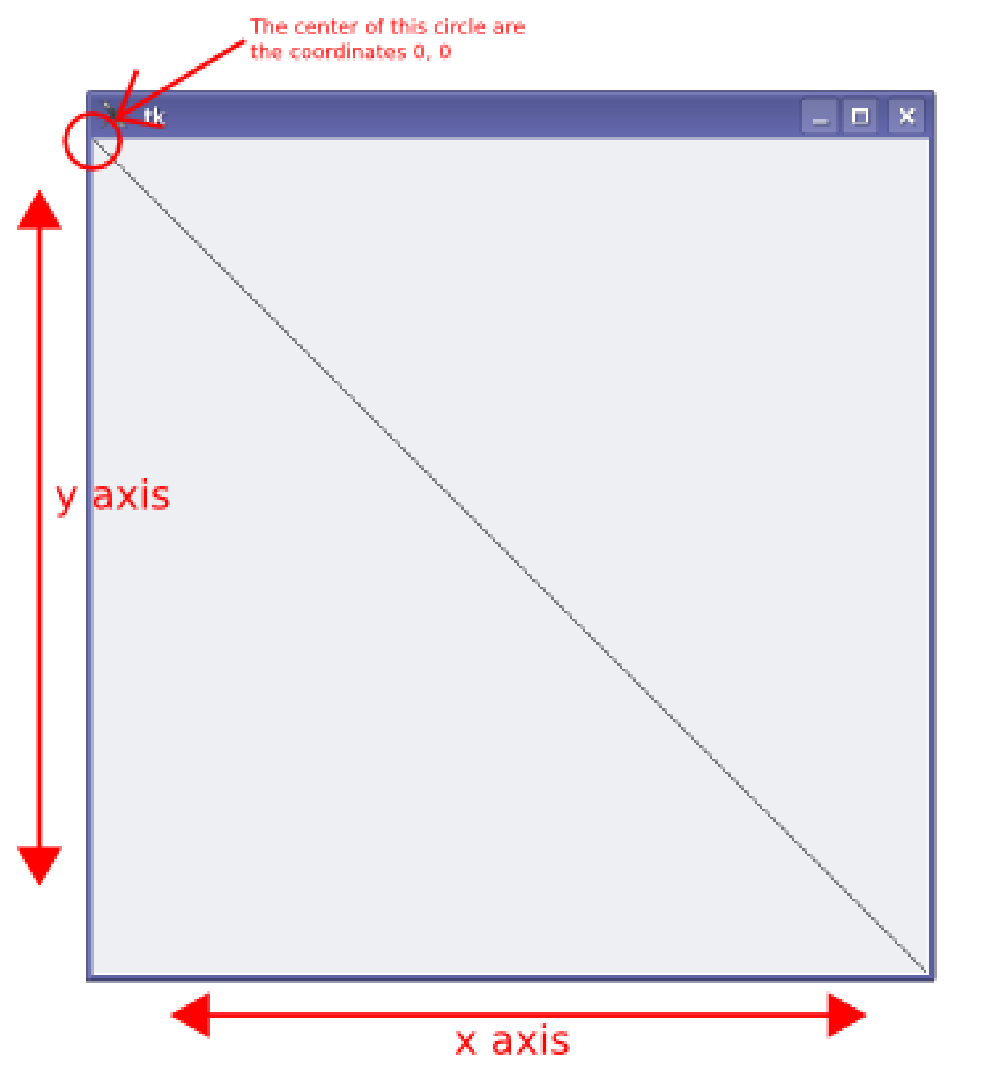
\includegraphics[width=80mm]{eps/figure32.eps}
\end{center}
\caption{Canvas x and y axis.}\label{fig32}
\end{figure}

Since the canvas is 500 pixels wide, and 500 pixels high, the coordinates of the bottom-right corner of the screen are 500,500. So the line in figure~\ref{fig32} can be drawn by using start coordinates of 0,0 and end coordinates of 500,500\index{modules!tkinter!create\_line}:

\begin{listing}
\begin{verbatim}
>>> from tkinter import *
>>> tk = Tk()
>>> canvas = Canvas(tk, width=500, height=500)
>>> canvas.pack()
>>> canvas.create_line(0, 0, 500, 500)
\end{verbatim}
\end{listing}

\noindent
Now, to do the same thing with turtle, would have required the following code:

\begin{listing}
\begin{verbatim}
>>> import turtle
>>> turtle.setup(width=500, height=500)
>>> t = turtle.Pen()
>>> t.up()
>>> t.goto(-250,250)
>>> t.down()
>>> t.goto(500,-500)
\end{verbatim}
\end{listing}

So the \code{tkinter} code is already an improvement, being shorter and less complicated. There are a large number of methods available on the canvas object, some of which aren't very useful to us, but let's take a look at some examples of the interesting functions.

\section{Drawing Boxes}

In turtle, we drew a box by moving forward, turning, moving forward, turning again and so on. Eventually you can draw a rectangular or square box, just by changing how far you move forward. With tkinter, drawing a square or rectangle is considerably easier---you just need to know the coordinates for the corners.

\begin{listingignore}
\begin{verbatim}
>>> from tkinter import *
>>> tk = Tk()
>>> canvas = Canvas(tk, width=400,height=400)
>>> canvas.pack()
>>> canvas.create_rectangle(10, 10, 50, 50)
1
\end{verbatim}
\end{listingignore}

In the above example, we create a canvas that is 400 pixels wide, and 400 pixels high, and then we draw a square in the top left corner (the top left corner is 10 pixels in from the top left, and and the bottom right corner is 50 pixels in from the bottom right). You might be wondering what the number is that appeared when you typed \code{create\_rectangle}\index{modules!tkinter!create\_rectange} and earlier when calling \code{create\_line}?  That's an identifying number for the shape you've just drawn (whether a line or a square or a circle). We'll come back to that number later.

The parameters that are passed to \code{create\_rectangle} are therefore: top left x position, top left y position, bottom right x position and bottom right y position. To save all that typing, we'll just refer to those as x1, y1 and x2, y2. We can draw a rectangle by making x2 a larger number:

\begin{listing}
\begin{verbatim}
>>> canvas.create_rectangle(100, 100, 300, 50)
\end{verbatim}
\end{listing}

\noindent
Or by making y2 a bit larger:

\begin{listing}
\begin{verbatim}
>>> canvas.create_rectangle(100, 200, 150, 350)
\end{verbatim}
\end{listing}

That last rectangle is basically saying: go 100 pixels across the canvas (from the top left), and 200 pixels down, then draw a box across to 150 pixels and down to 350 pixels. At the moment you should have something like figure~\ref{fig33} on your canvas.

\begin{figure}
\begin{center}
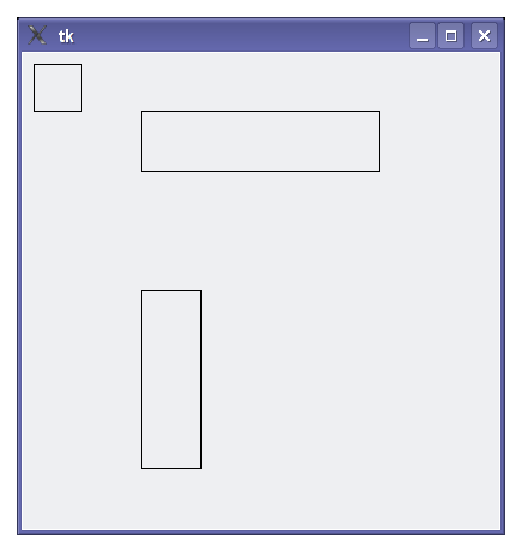
\includegraphics[width=80mm]{eps/figure33.eps}
\end{center}
\caption{tkinter boxes.}\label{fig33}
\end{figure}

Let's try filling the canvas with different sized rectangles. We can do this using a module called \code{random}\index{modules!random}. First import the random module:

\begin{listing}
\begin{verbatim}
>>> import random
\end{verbatim}
\end{listing}

Then we can create a function using a random number for the coordinates at the top and bottom corners.  The function to use is called \code{randrange}\index{modules!random!randrange}:

\begin{listing}
\begin{verbatim}
>>> def random_rectangle(width, height):
...     x1 = random.randrange(width)
...     y1 = random.randrange(height)
...     x2 = random.randrange(x1 + random.randrange(width))
...     y2 = random.randrange(y1 + random.randrange(height))
...     canvas.create_rectangle(x1, y1, x2, y2)
\end{verbatim}
\end{listing}

In the first two lines we create variables for the top left corner of the rectangle using \code{randrange}, passing the width and the height.  The \code{randrange} function takes a number as an argument (actually, see Appendix~\ref{app:afewpythonmodules} for more uses of \code{randrange})---so \code{randrange(10)} gives you a number between 0 and 9, \code{randrange(100)} gives you a number between 0 and 99, and so on. The next two lines create variables for the bottom right corner of the rectangle (or square!)---we use the top left coordinate (x1 or y1) and add a random number to that variable. Finally we call the \code{create\_rectangle} function using those variables. You can try out the \code{random\_rectangle} function by passing the width and height of the canvas you created:

\begin{listing}
\begin{verbatim}
>>> random_rectangle(400, 400)
\end{verbatim}
\end{listing}

\noindent
Or to fill the screen, how about creating a loop to call it a number of times:

\begin{listing}
\begin{verbatim}
>>> for x in range(0, 100):
...     random_rectangle(400, 400)
\end{verbatim}
\end{listing}

\noindent
Which produces a bit of a mess (figure~\ref{fig34}, but is interesting nonetheless.

\begin{figure}
\begin{center}
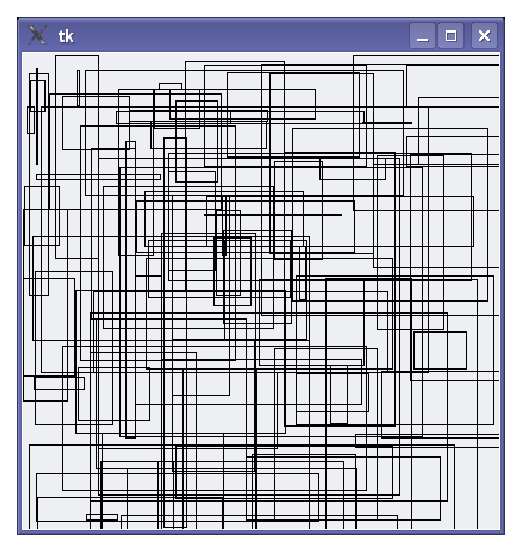
\includegraphics[width=80mm]{eps/figure34.eps}
\end{center}
\caption{A mess of rectangles.}\label{fig34}
\end{figure}

Remember, back in the last chapter, we set the colour the turtle drew with using percentages of the 3 colours: red, green and blue? With \code{tkinter} you can set the colour using similar ideas, but unfortunately, it's slightly more complicated than with \code{turtle}.  First of all, let's change the random rectangle function to pass in a colour to fill the rectangle with:

\begin{listing}
\begin{verbatim}
>>> def random_rectangle(width, height, fill_colour):
...     x1 = random.randrange(width)
...     y1 = random.randrange(height)
...     x2 = random.randrange(x1 + random.randrange(width))
...     y2 = random.randrange(y1 + random.randrange(height))
...     canvas.create_rectangle(x1, y1, x2, y2, fill=fill_colour)
\end{verbatim}
\end{listing}

The canvas \code{create\_rectangle} function can take a parameter `fill' which specifies the fill colour.  We can now pass this into the function. Try the following:

\begin{listing}
\begin{verbatim}
>>> random_rectangle(400, 400, 'green')
>>> random_rectangle(400, 400, 'red')
>>> random_rectangle(400, 400, 'blue')
>>> random_rectangle(400, 400, 'orange')
>>> random_rectangle(400, 400, 'yellow')
>>> random_rectangle(400, 400, 'pink')
>>> random_rectangle(400, 400, 'purple')
>>> random_rectangle(400, 400, 'violet')
>>> random_rectangle(400, 400, 'magenta')
>>> random_rectangle(400, 400, 'cyan')
\end{verbatim}
\end{listing}

Some, and maybe all, of those named colours will work.  But some of them might result in an error message (it depends on whether you're using Windows, Mac OS X or Linux). So far, that's pretty easy.  But what about a colour like gold?  In the \code{turtle} module, we created gold using 100\% of red, 85\% of green and no blue.  In \code{tkinter} we can create gold using:

\begin{listing}
\begin{verbatim}
>>> random_rectangle(400, 400, '#ffd800')
\end{verbatim}
\end{listing}

Which, all in all, is a pretty strange way to create a colour.  `ffd800' is called hexadecimal\index{hexadecimal colors}, and is another way to represent numbers.  Explaining how hexadecimal numbers work would take a few more pages than we have to spare for this book, so for the moment, you can use the following function to create a hexadecimal colour:

\begin{listing}
\begin{verbatim}
>>> def hexcolor(red, green, blue):
...     red = 255*(red/100.0)
...     green = 255*(green/100.0)
...     blue = 255*(blue/100.0)
...     return '#%02x%02x%02x' % (red, green, blue)
\end{verbatim}
\end{listing}

Calling hexcolor with 100\% for red, 85\% for green and 0\% for blue, results in the hexadecimal for a gold colour we just used:

\begin{listing}
\begin{verbatim}
>>> print(hexcolor(100, 85, 0))
#ffd800
\end{verbatim}
\end{listing}

\noindent
You can create a bright purple colour using 98\% of red, 1\% of green, and 77\% of blue:

\begin{listing}
\begin{verbatim}
>>> print(hexcolor(98, 1, 77))
#f902c4
\end{verbatim}
\end{listing}

\noindent
You can use that with the random\_rectangle function we created earlier:

\begin{listing}
\begin{verbatim}
>>> random_rectangle(400, 400, hexcolor(98, 1, 77))
\end{verbatim}
\end{listing}

\begin{figure}
\begin{center}
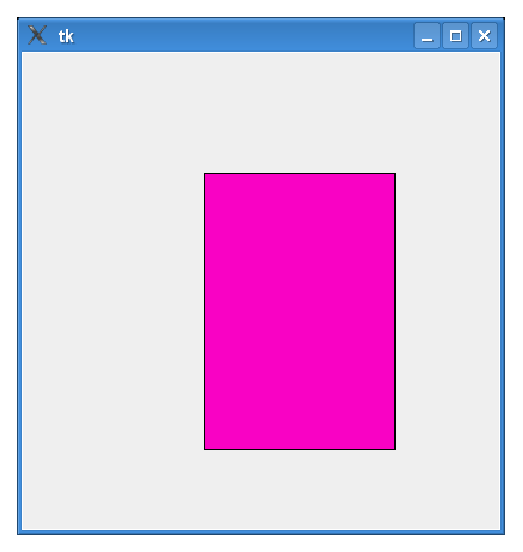
\includegraphics[width=80mm]{eps/figure35.eps}
\end{center}
\caption{A purple rectangle.}\label{fig35}
\end{figure}

\section{Drawing Arcs}

An arc is a part of a circle, but to draw one with tkinter you need to draw a rectangle. Which doesn't make a lot of sense until you try to draw a rectangle and then draw an arc inside it (see figure~\ref{fig36}). The code to draw this arc might look something like this\index{modules!tkinter!create\_arc}:

\begin{listing}
\begin{verbatim}
canvas.create_arc(10, 10, 200, 100, extent=180, style=ARC)
\end{verbatim}
\end{listing}

\begin{figure}
\begin{center}
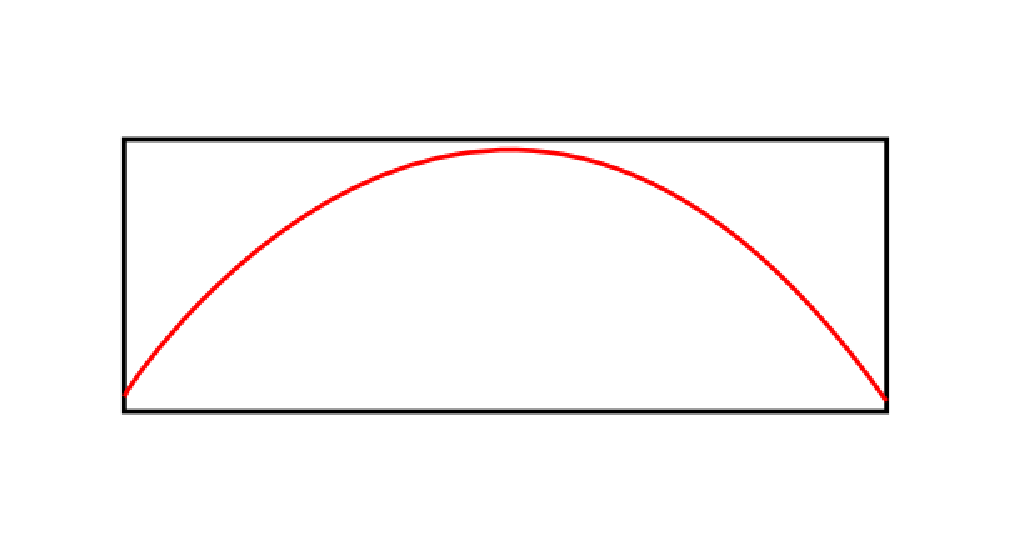
\includegraphics[width=80mm]{eps/figure36.eps}
\end{center}
\caption{An arc fitting inside a rectangle.}\label{fig36}
\end{figure}

This places the top left corner of the rectangle at the coordinates 10, 10 (that's 10 pixels across, 10 pixels down), and the bottom right corner of the rectangle at the coordinates 200, 100 (200 pixels across, 100 pixels down).  The next parameter (a \textbf{named} parameter) `extent' is used to specify the degrees of the angle of the arc.  If you don't know anything about degrees in a circle (or arc), then just remember that if you think about a circle, 180 degrees would be half of the circle (or half the arc), 359 degrees would be a full circle, 90 degrees is a quarter of a circle and 0 degrees is$\ldots$ well, nothing at all. Here's some code that draws a bunch of different arcs down the page so you can see the basic differences when we use different degrees (you can see the examples in figure~\ref{fig37}):

\begin{listing}
\begin{verbatim}
>>> canvas.create_arc(10, 10, 200, 80, extent=45, style=ARC)
>>> canvas.create_arc(10, 80, 200, 160, extent=90, style=ARC)
>>> canvas.create_arc(10, 160, 200, 240, extent=135, style=ARC)
>>> canvas.create_arc(10, 240, 200, 320, extent=180, style=ARC)
>>> canvas.create_arc(10, 320, 200, 400, extent=359, style=ARC)
\end{verbatim}
\end{listing}

\begin{figure}
\begin{center}
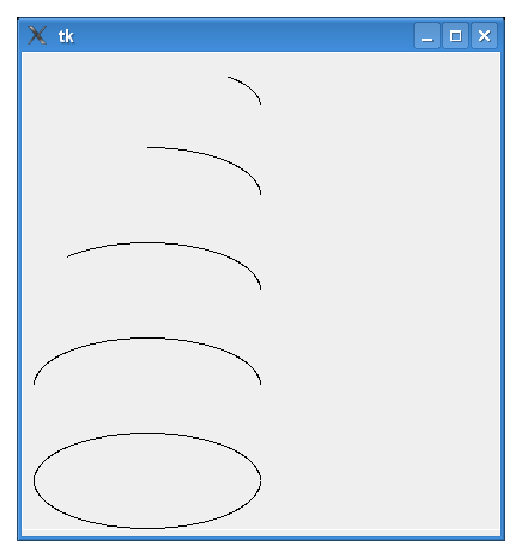
\includegraphics[width=80mm]{eps/figure37.eps}
\end{center}
\caption{Differing degrees of arcs.}\label{fig37}
\end{figure}

\section{Drawing Ovals}

While the last statement in the above example draws an oval, you can also draw ovals using the \code{create\_oval}\index{modules!tkinter!create\_oval} function.  Similar to drawing arcs, an oval is drawn inside the boundaries of a rectangle. For example, the following code:

\begin{listing}
\begin{verbatim}
>>> tk = Tk()
>>> canvas = Canvas(tk, width=400,height=400)
>>> canvas.pack()
>>> canvas.create_oval(1, 1, 300, 200)
\end{verbatim}
\end{listing}

This example draws an oval in the (imaginary) square drawn from pixel positions 1,1 to 300,200. If we draw a red rectangle with the same coordinates, you can properly see how the oval is drawn inside (figure~\ref{fig38}):

\begin{listing}
\begin{verbatim}
>>> canvas.create_rectangle(1, 1, 300, 200, outline="#ff0000")
\end{verbatim}
\end{listing}

\begin{figure}
\begin{center}
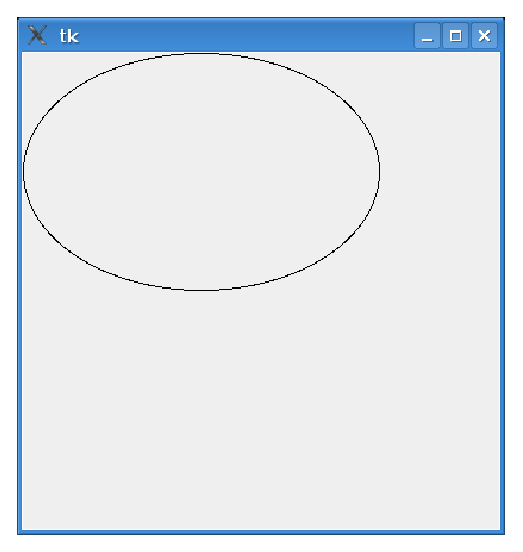
\includegraphics[width=80mm]{eps/figure38.eps}
\end{center}
\caption{The outline of an oval.}\label{fig38}
\end{figure}

\begin{figure}
\begin{center}
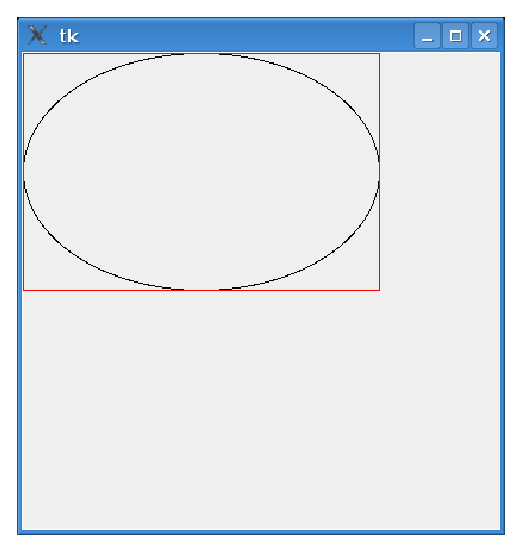
\includegraphics[width=80mm]{eps/figure39.eps}
\end{center}
\caption{The outline of an oval inside a rectangle.}\label{fig39}
\end{figure}

\noindent
To draw a circle, rather than an elliptical oval, the imaginary rectangle should be a square (which produces the circle in figure~\ref{fig40}):

\begin{listing}
\begin{verbatim}
>>> tk = Tk()
>>> canvas = Canvas(tk, width=400,height=400)
>>> canvas.pack()
>>> canvas.create_oval(1, 1, 300, 300)
\end{verbatim}
\end{listing}

\begin{figure}
\begin{center}
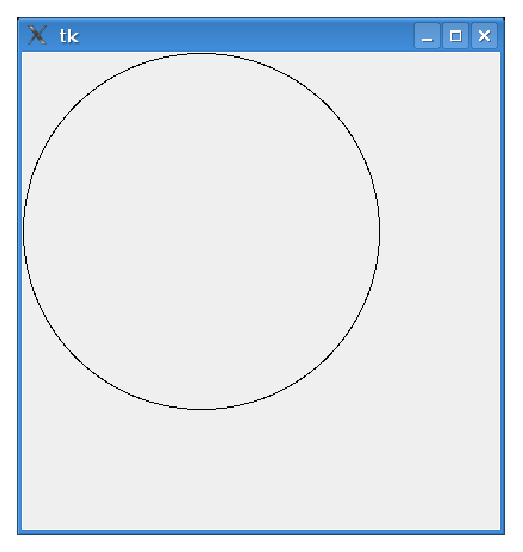
\includegraphics[width=80mm]{eps/figure40.eps}
\end{center}
\caption{A simple circle.}\label{fig40}
\end{figure}

\section{Drawing Polygons}\index{modules!tkinter!create\_polygon}

A polygon is any shape with 3 or more sides. Triangles, squares, rectangles, pentagons, hexagons, and so on are all examples of polygons. As well as these more regular shapes, you can also create irregular shaped polygons. For example, to draw a triangle, you need to provide 3 sets of coordinates (that's a position across plus a position down) for each point of the triangle (creating the triangle in figure~\ref{fig41}):

\begin{listing}
\begin{verbatim}
>>> from tkinter import *
>>> tk = Tk()
>>> canvas = Canvas(tk, width=400,height=400)
>>> canvas.pack()
>>> canvas.create_polygon(10, 10, 100, 10, 100, 50, fill="", outline="black")
\end{verbatim}
\end{listing}

\begin{figure}
\begin{center}
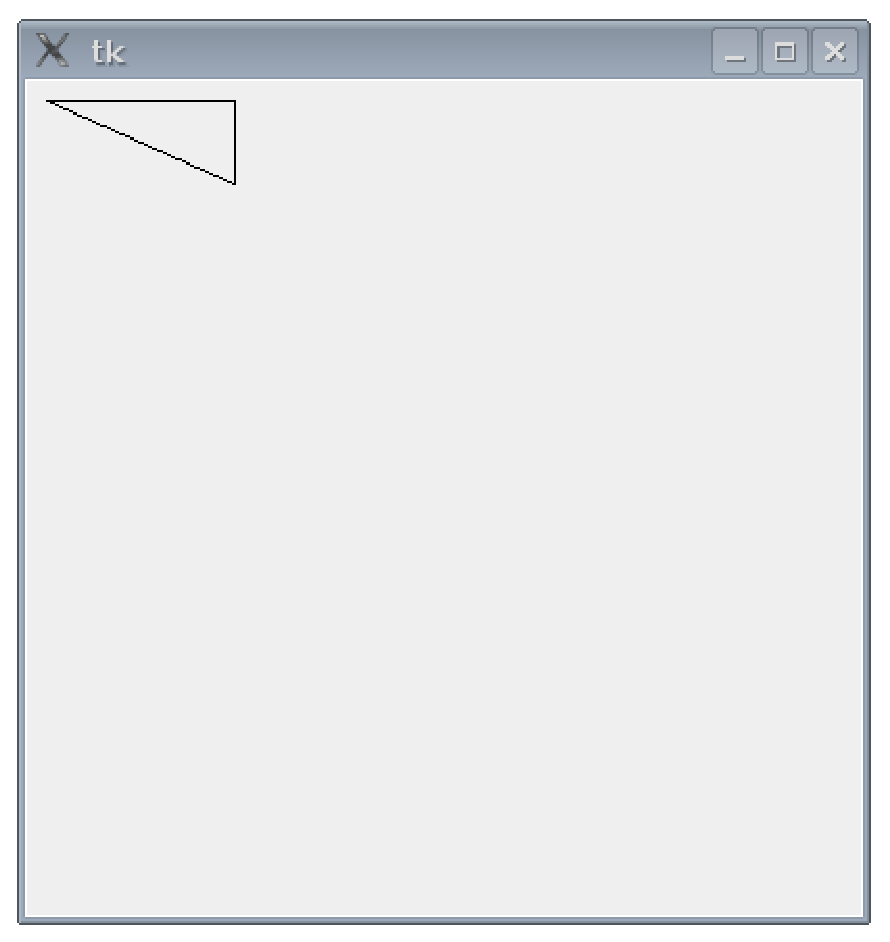
\includegraphics[width=80mm]{eps/figure41.eps}
\end{center}
\caption{A simple triangle.}\label{fig41}
\end{figure}

We can add an irregular polygon using the following code. Figure~\ref{fig42} shows both the triangle and the oddly shaped polygon.

\begin{listing}
\begin{verbatim}
>>> canvas.create_polygon(200, 10, 240, 30, 120, 100, 140, 120, fill="", outline="black")
\end{verbatim}
\end{listing}

\begin{figure}
\begin{center}
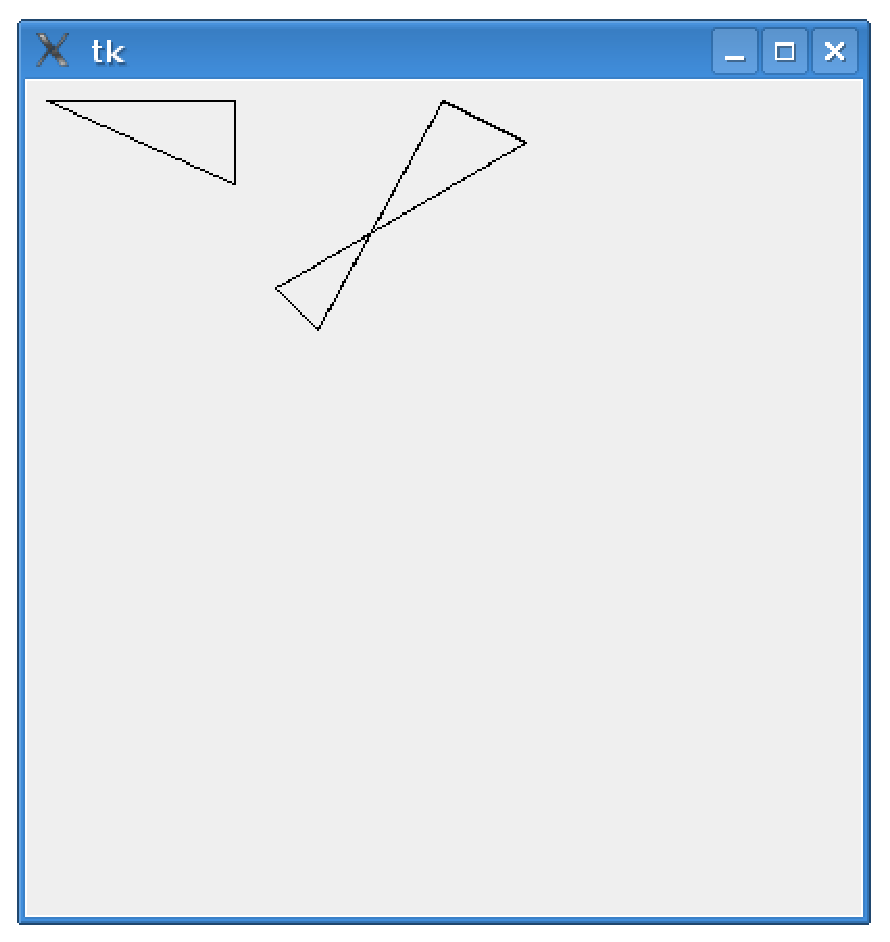
\includegraphics[width=80mm]{eps/figure42.eps}
\end{center}
\caption{A simple triangle.}\label{fig42}
\end{figure}

\section{Drawing Images}

You can draw an image on a canvas using \code{tkinter} by first loading the image, then using the \code{create\_image}\index{modules!tkinter!create\_image} function on the canvas object. This sounds a bit illogical, but it works as follows:

\begin{listing}
\begin{verbatim}
1. >>> from tkinter import *
2. >>> tk = Tk()
3. >>> canvas = Canvas(tk, width=400, height=400)
4. >>> canvas.pack()
5. >>> myimage = PhotoImage(file='test.gif')
6. >>> canvas.create_image(0, 0, image=myimage, anchor=NW)
\end{verbatim}
\end{listing}

In lines 1 to 4 we set up the canvas the same as we have in previous examples. In line 5, the image is loaded into the variable \code{myimage}. It's important that the image you want to load is in a directory that's accessible to Python. This is usually the directory that the Python console is running from. You can find out the name of this directory by importing the \code{os}\index{modules!os} module and using the \code{getcwd()} function:

\begin{listing}
\begin{verbatim}
>>> import os
>>> print(os.getcwd())
\end{verbatim}
\end{listing}

\begin{WINDOWS}
This will probably print out something like `c:\\Python30'.
\end{WINDOWS}

\begin{MAC}
This will probably print out something like `/Users/yourname'$\ldots$, so if your name is Jane Matthews, \code{getcwd()} might return `/Users/janematthews'.
\end{MAC}

\begin{LINUX}
This will probably print out something like `/home/yourname'$\ldots$, so if your name is Jane Matthews, \code{getcwd()} might return `/home/jane' or `/home/janematthews', depending upon how your computer has been setup.
\end{LINUX}

Copy your image into that directory and then load it using the PhotoImage function (same as line 5). You then use the \code{create\_image} function on the canvas to display your image (line 6). If you've done all this correctly, you'll see something like figure~\ref{fig43}.

\begin{figure}
\begin{center}
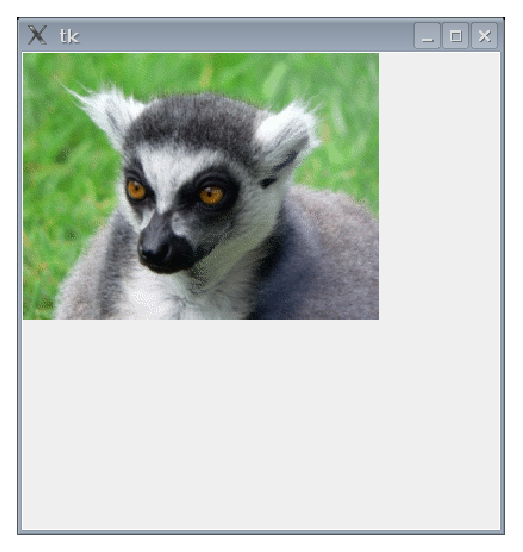
\includegraphics[width=80mm]{eps/figure43.eps}
\end{center}
\caption{A photo image.}\label{fig43}
\end{figure}

PhotoImage can load image files with the extensions .gif, .ppm and .pgm. If you want to load other types of images (there are lots of different ways you can create image files---for example, digital cameras usually store images with the extension .jpg), then you'll need to use an extension which adds that capability to Python. The Python Imaging Library (PIL)\footnote{The Python Imaging Library can be found at \href{http://www.pythonware.com/products/pil/index.htm}{http://www.pythonware.com/products/pil/index.htm}} adds the ability to load all kinds of images, as well as do things like expand and shrink, change image colours, reverse images and so on. However, installing and using the Python Imaging Library, is a bit beyond the scope of this book.

\section{Basic Animation}\index{modules!tkinter!basic animation}

So far, we've seen how to do static drawing---that's pictures that don't move. What about animation? Animation is not necessarily \code{Tk}'s strong suit, but you can do the basics. For example, we can create a filled triangle and then make it move across the screen using the following code:

\begin{listingignore}
\begin{verbatim}
1.  >>> import time
2.  >>> from tkinter import *
3.  >>> tk = Tk()
4.  >>> canvas = Canvas(tk, width=400, height=400)
5.  >>> canvas.pack()
6.  >>> canvas.create_polygon(10, 10, 10, 60, 50, 35)
7.  1
8.  >>> for x in range(0, 60):
9.  ...     canvas.move(1, 5, 0)
10. ...     tk.update()
11. ...     time.sleep(0.05)
\end{verbatim}
\end{listingignore}

The moment you press the Enter key after typing the last line, the triangle will start moving across the screen (you can see it half-way across in figure~\ref{fig44}).

\begin{figure}
\begin{center}
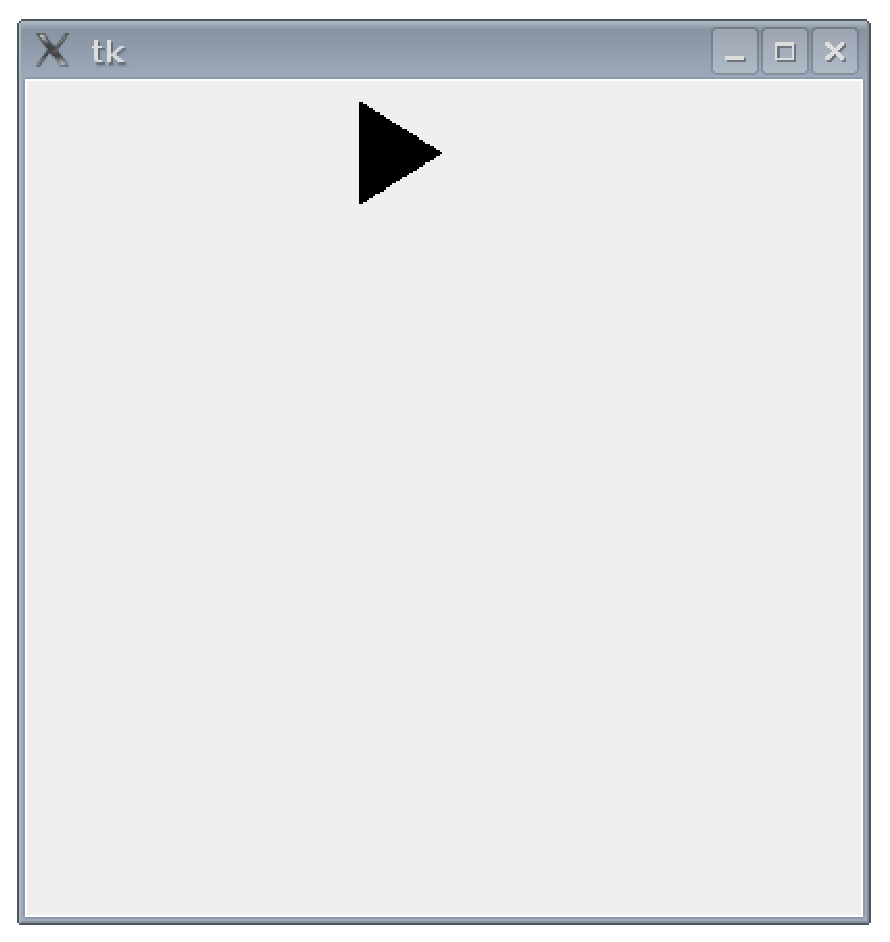
\includegraphics[width=80mm]{eps/figure44.eps}
\end{center}
\caption{The triangle moving across the screen.}\label{fig44}
\end{figure}

\par
\emph{How does it work?}
\par
Lines 1 to 5 we've seen before---it's just the basic setup to display a canvas---and in line 6, we create the triangle (using the \code{create\_polygon} function), and in line 7 you can see the identifier (the number 1) that is returned by this function. In line 8, we setup a simple for-loop to count from 0 to 59.

The block of lines (9 to 11) is the code to move the triangle. The \code{move} function on the canvas object will move any drawn object by adding values to the object's x and y coordinates. For example, in line 9 we move the object with id 1 (the identifier for the triangle) 5 pixels across and 0 pixels down. If we wanted to move the back again we might use canvas.move(1, -5, 0)\index{modules!tkinter!move}.
 
The function \code{update} on the \code{tk} object forces it to update (if we didn't use \code{update}, tkinter would wait until the loop had finished before moving the triangle, which means you wouldn't see it move). Finally line 11 tells Python to sleep for 1/20th of a second (0.05), before continuing. We can change this code, so the triangle moves diagonally down the screen, by calling \code{move(1, 5, 5)}.  First, close the canvas (by clicking on the X button on the window), then try this code:

\begin{listingignore}
\begin{verbatim}
>>> import time
>>> tk = Tk()
>>> canvas = Canvas(tk, width=400, height=400)
>>> canvas.pack()
>>> canvas.create_polygon(10, 10, 10, 60, 50, 35)
1
>>> for x in range(0, 60):
...     canvas.move(1, 5, 5)
...     tk.update()
...     time.sleep(0.05)
...
\end{verbatim}
\end{listingignore}

Figure~\ref{fig45} shows the triangle part way down the screen. Move the triangle diagonally back up the screen to its starting position, by using -5, -5:

\begin{listing}
\begin{verbatim}
>>> import time
>>> for x in range(0, 60):
...     canvas.move(1, -5, -5)
...     tk.update()
...     time.sleep(0.05)
\end{verbatim}
\end{listing}

\begin{figure}
\begin{center}
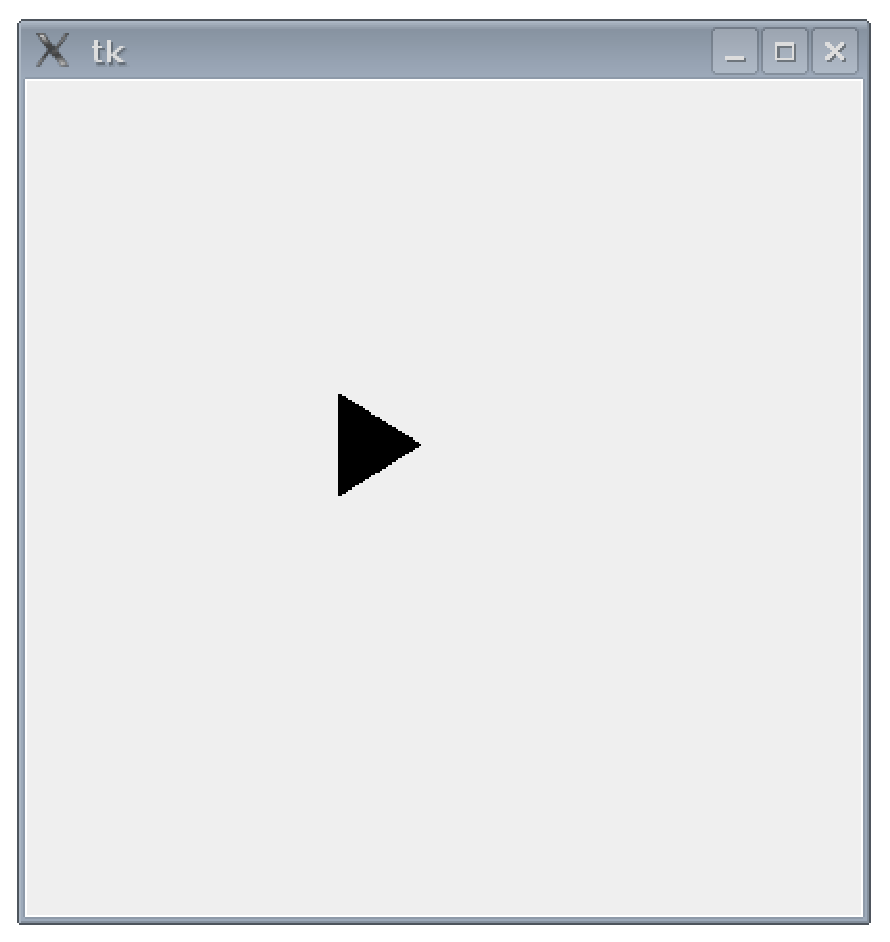
\includegraphics[width=80mm]{eps/figure45.eps}
\end{center}
\caption{The triangle moving down the screen.}\label{fig45}
\end{figure}

\section{Reacting to events$\ldots$}\index{modules!tkinter!events}

We can also make the triangle react when someone hits a key, by using what are called \emph{event bindings}.  Events are things that occur while a program is running, such as someone moving the mouse, hitting a key, or even closing a window. You can setup \code{Tk} to look out for these events, and then do something in response. To begin handling events we need to start by creating a function. Suppose we want the triangle to move when the enter key is pressed? We can define a function to move the triangle:

\begin{listing}
\begin{verbatim}
>>> def movetriangle(event):
...     canvas.move(1, 5, 0)
\end{verbatim}
\end{listing}

The function needs to have a single parameter (event), which is used by Tk to send information to the function about what has happened.  We then tell Tk that this function should be used for a particular event, using the \code{bind\_all}\index{modules!tkinter!bind\_all} function on the canvas. The full code looks like this:

\begin{listing}
\begin{verbatim}
>>> from tkinter import *
>>> tk = Tk()
>>> canvas = Canvas(tk, width=400, height=400)
>>> canvas.pack()
>>> canvas.create_polygon(10, 10, 10, 60, 50, 35)
>>> def movetriangle(event):
...     canvas.move(1, 5, 0)
...
>>> canvas.bind_all('<KeyPress-Return>', movetriangle)
\end{verbatim}
\end{listing}

The first parameter in the \code{bind\_all} function describes the event which we want Tk to look out for. In this case, it's the event \code{<KeyPress-Return>} (which is a press of the enter key).  We tell Tk that the \code{movetriangle} function should be called when this key-press event occurs.  If you run this code, click on the Tk canvas with your mouse, and then try hitting the Enter (or Return) key on your keyboard.

How about changing the direction of the triangle depending upon different key presses, such as the arrow keys? First of all we change the \code{move} triangle function to the following:

\begin{listing}
\begin{verbatim}
>>> def movetriangle(event):
...     if event.keysym == 'Up':
...         canvas.move(1, 0, -3)
...     elif event.keysym == 'Down':
...         canvas.move(1, 0, 3)
...     elif event.keysym == 'Left':
...         canvas.move(1, -3, 0)
...     else:
...         canvas.move(1, 3, 0)
\end{verbatim}
\end{listing}

The event object that is passed to \code{movetriangle}, contains a number of \emph{properties}\footnote{Properties are named values, which describe something---for example, a property of the sky is that it's blue (sometimes), a property of a car is that it has wheels. In programming terms, a property has a name and a value.}.  One of these properties is \code{keysym}, which is a string holding the value of the actual key pressed.  If \code{keysym} contains the string `Up', we call \code{canvas.move} with the parameters (1, 0, -3); if it contains down we call with the parameters (1, 0, 3), and so on.  Remember that the first parameter is the identifying number for the shape drawn on the canvas, the second parameter is the value to add to the x (horizontal) coordinate, and the last parameter is the value to add to the y (vertical) coordinate. We then tell Tk that the \code{movetriangle} function should be used to handle events from 4 different keys (up, down, left and right).  So, the code now looks like this:

\begin{listingignore}
\begin{verbatim}
>>> from tkinter import *
>>> tk = Tk()
>>> canvas = Canvas(tk, width=400, height=400)
>>> canvas.pack()
>>> canvas.create_polygon(10, 10, 10, 60, 50, 35)
1 
>>> def movetriangle(event):
...     if event.keysym == 'Up':
...         canvas.move(1, 0, -3)
...     elif event.keysym == 'Down':
...         canvas.move(1, 0, 3)
...     elif event.keysym == 'Left':
...         canvas.move(1, -3, 0)
...     else:
...         canvas.move(1, 3, 0)
... 
>>> canvas.bind_all('<KeyPress-Up>', movetriangle)
>>> canvas.bind_all('<KeyPress-Down>', movetriangle)
>>> canvas.bind_all('<KeyPress-Left>', movetriangle)
>>> canvas.bind_all('<KeyPress-Right>', movetriangle)
\end{verbatim}
\end{listingignore}

\noindent
With this example, the triangle now moves in the direction of the arrow key that you press.

\newpage
